\subsection{Overview}

The framework assumes that 100\% burnt area occurs in perfect fire conditions,  i.e. complete fuel coverage, no moisture, saturated ignition and no agricultural or urban fragmentation. This is analogous to the dry season in tropical savanna and grasslands \citep{kelley2014modelling}, particularly parts of Northern Australia \citep{murphy2013fire} and the Sahel \citep{van2008climate} which experience complete buring each year.
Burnt area is reduced as each control becomes sub-optimal, i.e.
    fuel loads become discontinuous  (e.g. desert areas)
    or too moist (e.g. Humid evergreen forests),
    if there is a lack of ignition (shown to influence interannual variability in parts Southern Australia \cite{bradstock2010biogeographic} \hlb{and probably some other places}),
    or with increased human influence on the landscape (e.g. cropland or urban areas).
Fractional burnt area ($F$) is the product of the maximum allowed burnt area for each control ($F_i$).
\begin{equation}
    F=\Pi_{i} F_i
    \label{equ:LimFIRE}
\end{equation}
\hlb{Is it widley known that $\Pi$ means product?}

A controls maximum burnt area is related to fuel loads, moisture, ignitions or suppression via the logistic function, as per \citet{bistinas2014causal}:

\begin{equation}
    f(x) = 1 / (1 + e^{-k \cdot (x - x_0)})
    \label{equ:fx}
\end{equation}
where $k$ described the steepness of the curve and $x_0$ is the curves midpoint (see figure ~\ref{fig:Logistic_fun}).

\begin{figure}[!ht]
  \centering
    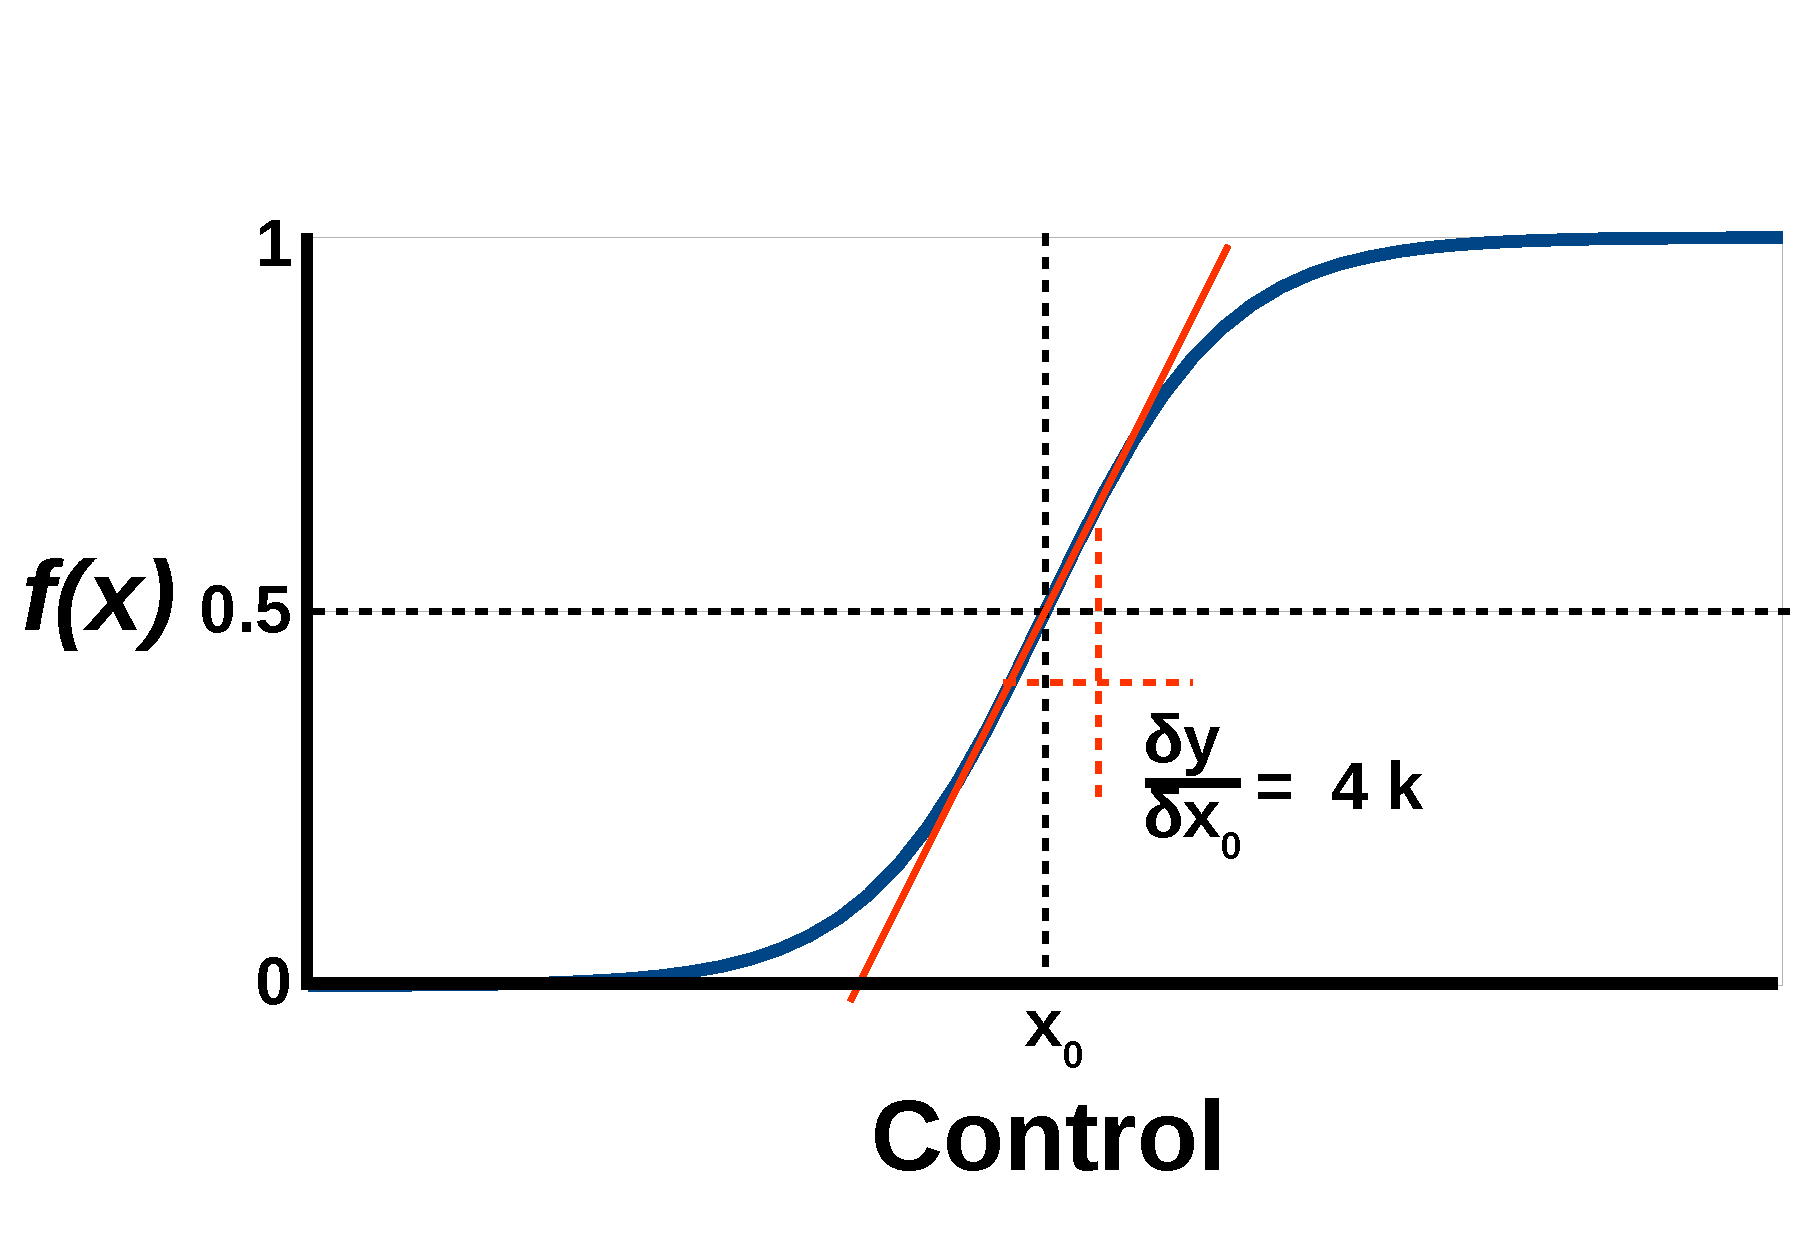
\includegraphics[width=0.67\textwidth]{diagrams/Logistic_fun.pdf}
  \caption{Logistic function.}
  \label{fig:Logistic_fun}
\end{figure}

Fire increases with increasing fuel load ($F_w$) and igntions ($F_{ig}$), and decreases with moisture ($F_{\omega}$) and anthropagenic supression ($F_s$). Therefore:

\begin{equation}
    \begin{split}
        F_{w} = f(w) \\
        F_{\omega} = 1 - f(\omega) \\
        F_{ig} = f(ig) \\
        F_{s} = 1- f(s)
    \end{split}
    \label{equ:LimFIRE.x}
\end{equation}

\begin{figure}[!ht]
  \centering
    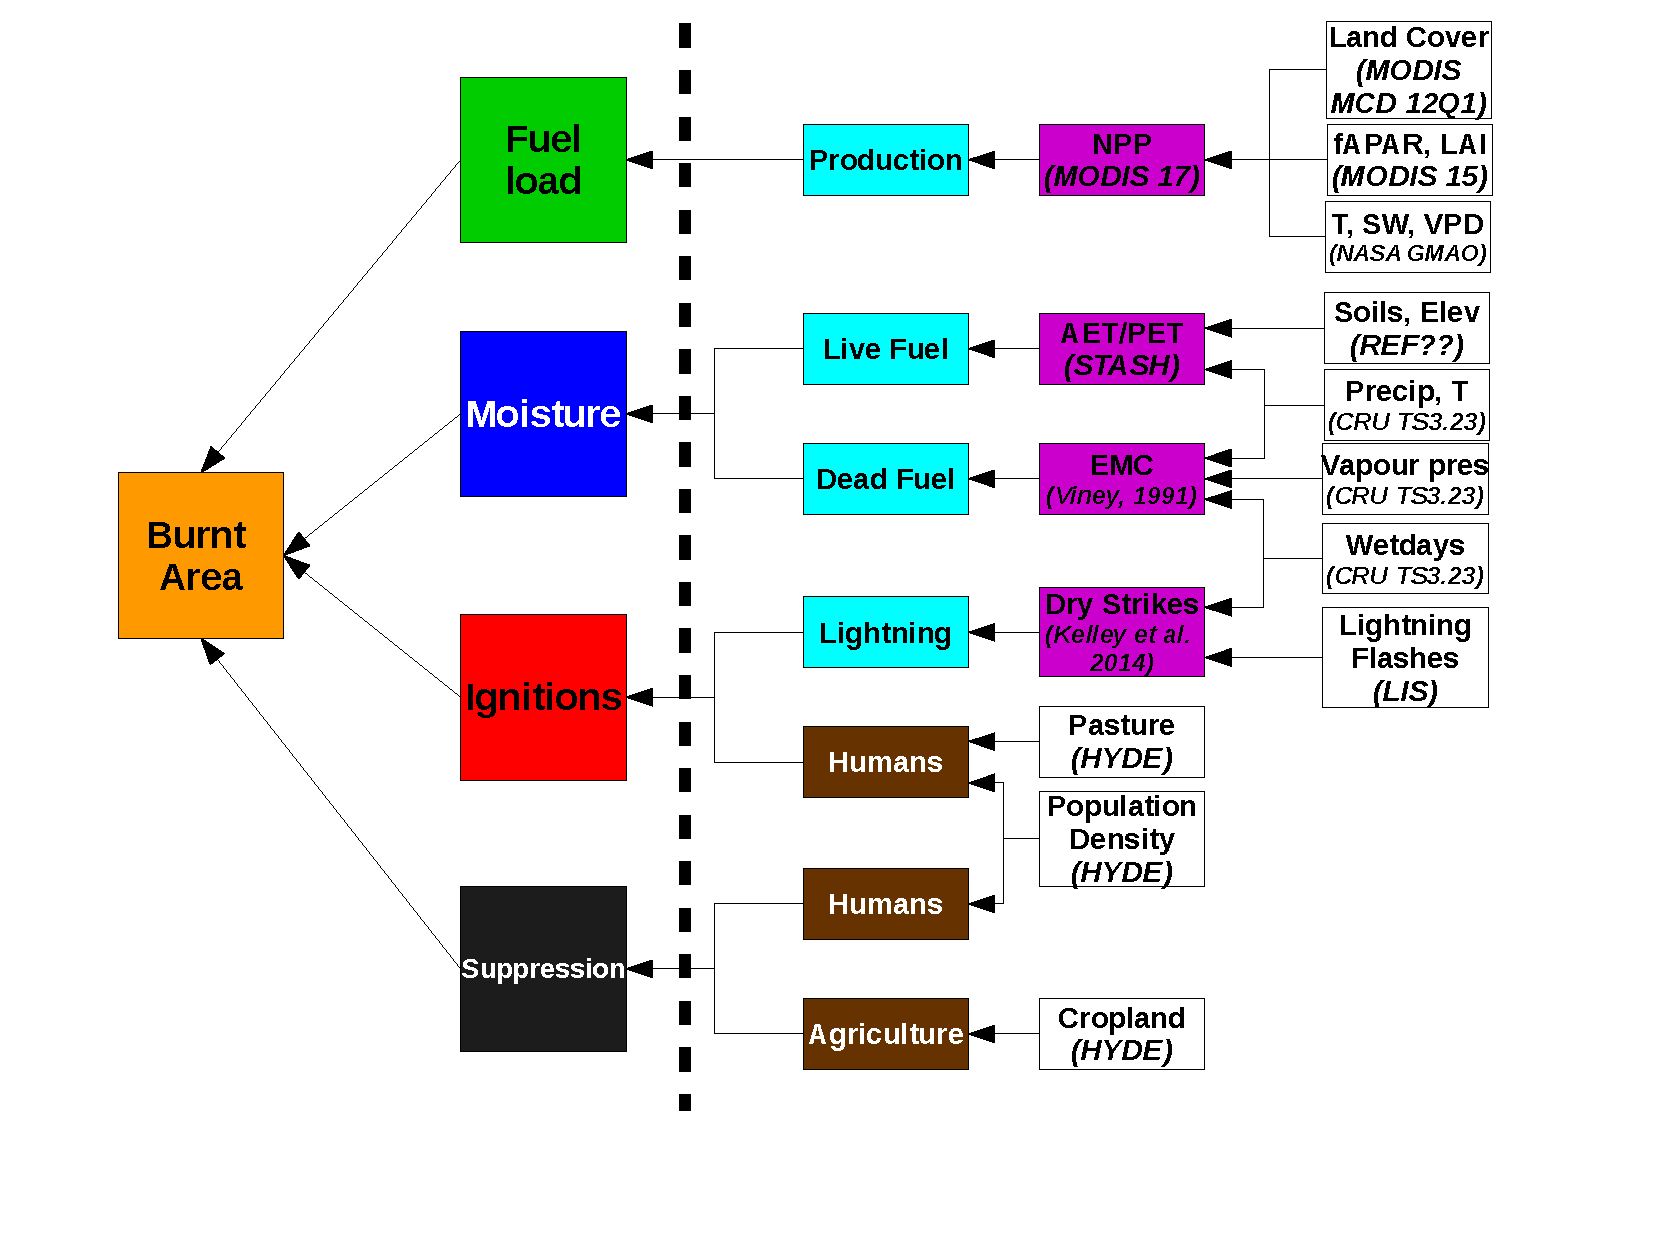
\includegraphics[width=0.8\textwidth]{diagrams/Model_schematic.pdf}
  \caption{Framework description.}
\end{figure}
